\section{\KLUDGE ディレクトリ構成}

\begin{figure}[t]
\begin{center}
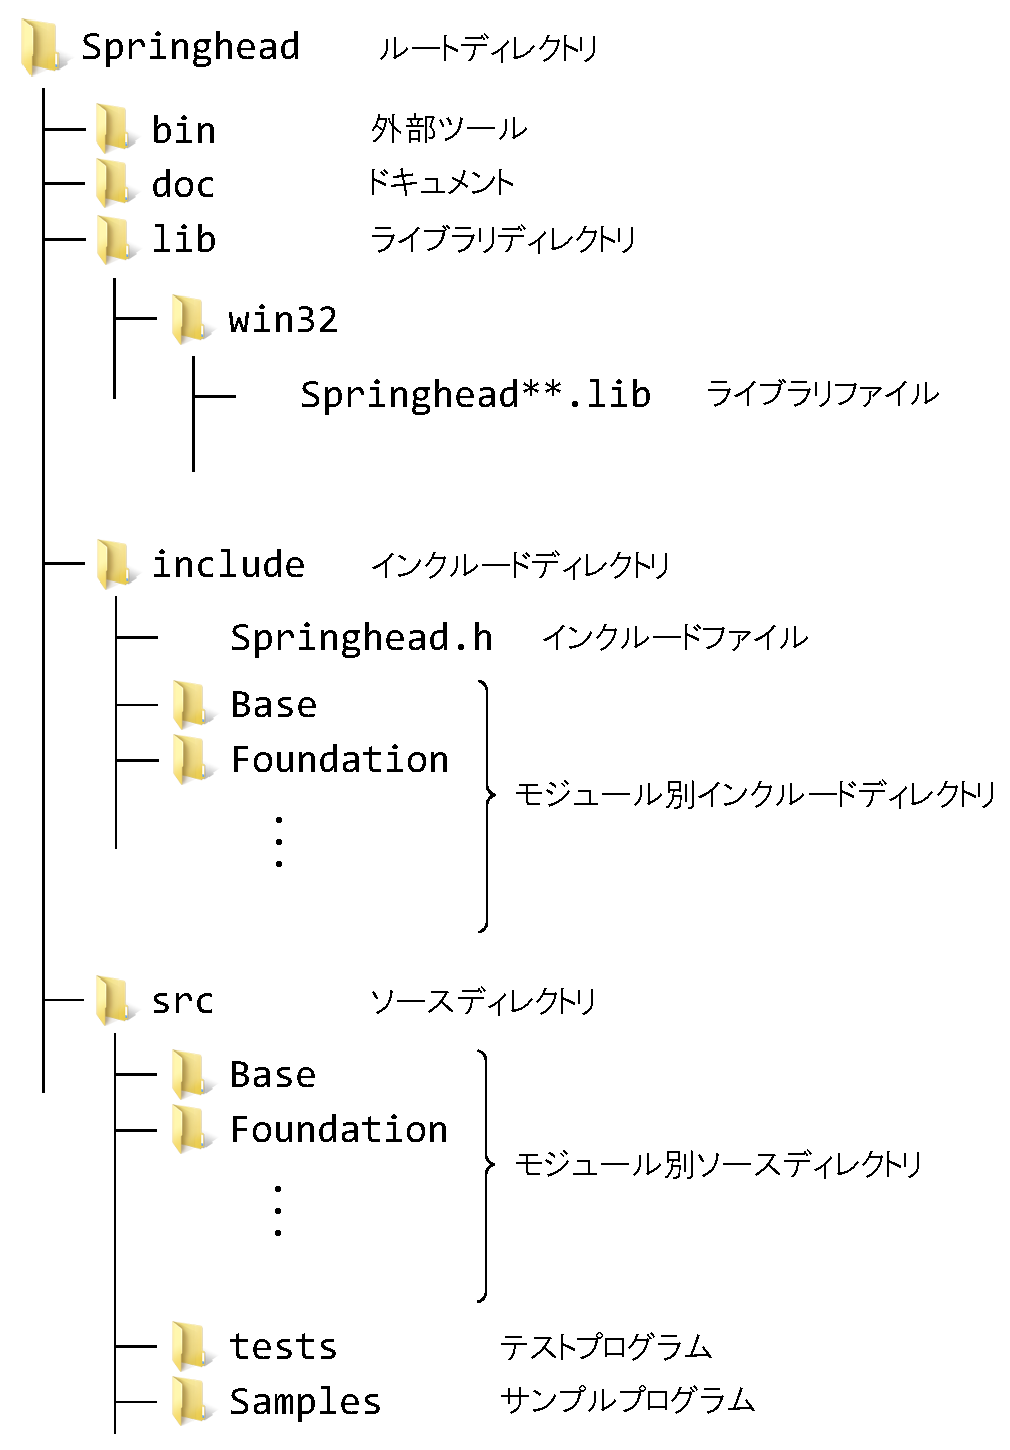
\includegraphics[width=.6\hsize]{fig/filetree.eps}
\end{center}
\caption{Directory tree of Springhead}
\label{fig_filetree}
\end{figure}

Springhead\KLUDGE のディレクトリ構成をFig.\,\ref{fig_filetree}\KLUDGE に示します.

\section{\KLUDGE ライブラリ構成}

\begin{table}[t]
\caption{Springhead modules}
\label{table_modules}
\begin{tabular}{lll}
\toprule
\KLUDGE モジュール名			& \KLUDGE プリフィックス	& \KLUDGE 機能	\\ \midrule
{\bf Base}				& -					& \KLUDGE 行列・ベクトル演算,スマートポインタ,\\
						&					& \KLUDGE その他基本機能	\\
{\bf Foundation}		& UT				& Springhead\KLUDGE の基本クラス,実行時型情報	\\
{\bf Collision}			& CD				& \KLUDGE 衝突判定	\\
{\bf Physics}			& PH				& \KLUDGE 物理計算	\\
{\bf Graphics}			& GR				& \KLUDGE シーングラフ,描画	\\
{\bf FileIO}			& FI				& \KLUDGE ファイル入出力	\\
{\bf HumanInterface}	& HI				& \KLUDGE ヒューマンインタフェースデバイスや \\
						&					& \KLUDGE インタラクション \\ 
{\bf Creature}			& CR				& \KLUDGE バーチャルクリーチャ \\
{\bf Framework}			& FW				& \KLUDGE モジュール間の連携と \\
						&					& \KLUDGE アプリケーション作成支援 \\ \bottomrule
\end{tabular}
\end{table}

\begin{table}[t]
\caption{Module dependencies}
\label{table_dependency}
\begin{center}
\begin{tabular}{llllllllll}
\toprule
\KLUDGE モジュール名			& 			&			&			&			&			&			&			&			&			\\ \midrule
{\bf Base}				& -			& -			& -			& -			& -			& -			& -			& -			& -			\\
{\bf Foundation}		& $\circ$	& -			& -			& -			& -			& -			& -			& -			& -			\\
{\bf Collision}			& $\circ$	& $\circ$	& -			& -			& -			& -			& -			& -			& -			\\
{\bf Physics}			& $\circ$	& $\circ$	& $\circ$	& -			& -			& -			& -			& -			& -			\\
{\bf Graphics}			& $\circ$	& $\circ$	& -			& -			& -			& -			& -			& -			& -			\\
{\bf FileIO}			& $\circ$	& $\circ$	& -			& -			& -			& -			& -			& -			& -			\\
{\bf HumanInterface}	& $\circ$	& $\circ$	& -			& -			& -			& -			& -			& -			& -			\\
{\bf Creature}			& $\circ$	& $\circ$	& -			& $\circ$	& -			& -			& -			& -			& -			\\
{\bf Framework}			& $\circ$	& $\circ$	& -			& $\circ$	& $\circ$	& $\circ$	& $\circ$	& -			& -			\\ \bottomrule
\end{tabular}
\end{center}
\end{table}

Springhead\KLUDGE は複数のモジュールから構成されています.
Table\,\ref{table_modules}\KLUDGE にモジュール一覧を示します.
Table\,\ref{table_dependency}\KLUDGE にモジュール間の依存関係を示します.
\KLUDGE 通常,ユーザはSpringhead\KLUDGE を使用するにあたってこれらの依存関係を陽に意識する必要はありません.
\KLUDGE また,何らかの事情でSpringhead\KLUDGE の特定の機能(たとえば物理シミュレーション)のみを用いたいという場合に対応できるように,
\KLUDGE モジュール間の依存関係はなるべく疎になるように設計されています.
\KLUDGE したがってこのような場合には用途に応じて必要なモジュールのみを使えるようになっています.

\section{\KLUDGE クラス・API\KLUDGE の命名規則}

\KLUDGE 各モジュールに含まれるクラスの名前には,Table\,\ref{table_modules}\KLUDGE に示されるようなモジュール固有のプリフィックスがつきます
(\KLUDGE 例: Physics\KLUDGE モジュールの\texttt{PHSolid}\KLUDGE ,Collision\KLUDGE モジュールの\texttt{CDShape})\KLUDGE .
\KLUDGE 一部にはこのルールにしたがわないクラスも存在します(\KLUDGE 例: Foundation\KLUDGE モジュールのObject)\KLUDGE .

API(\KLUDGE クラスのメンバ関数)\KLUDGE にも緩い命名規則があります.
API\KLUDGE 名は基本的に(\KLUDGE 動詞 + \KLUDGE 目的語)\KLUDGE という形式で処理内容を端的に表現します.
\KLUDGE また,単語の先頭文字のみ大文字,その他は小文字で表記します.
\KLUDGE 例としては\texttt{PHSolid::SetMass}\KLUDGE ,\texttt{GRSdk::CreateScene}\KLUDGE などです.

\section{\KLUDGE インタフェースとディスクリプタ} 
\label{sec_if_desc}

Springhead\KLUDGE では仕様と実装を明確に分離するために,インタフェースクラスと実装クラスが分けられています.
\KLUDGE ユーザはインタフェースクラスのみを使用してSpringhead\KLUDGE の機能を利用します.
\KLUDGE ただし,\url{Base}\KLUDGE と\url{Foundation}\KLUDGE モジュールにあるごく基本的なクラス,および\url{Framework}\KLUDGE のアプリケーションクラスは例外となっています.

\KLUDGE また,Springhead\KLUDGE のクラスにはそれぞれにディスクリプタが用意されています.ディスクリプタとは,そのクラスの読み書き可能な属性のみを集めた構造体です.
\KLUDGE ディスクリプタを利用することで,同じ設定のインスタンスを多数設定することが用意になります.
\KLUDGE また,ディスクリプタはファイルへのデータの保存や読み込みにおいても役立ちます.

\KLUDGE 以下に\url{Physics}\KLUDGE モジュールの剛体を表す\url{PHSolid}\KLUDGE クラスを例にとって説明します.
\begin{sourcecode}
// given PHSolidIf* phScene, 

PHSolidDesc desc;
desc.mass = 1.0;

PHSolidIf* solid = phScene->CreateSolid(desc);
\end{sourcecode}
\KLUDGE 上のコードで\url{PHSolidDesc}\KLUDGE は\url{PHSolid}\KLUDGE クラスのディスクリプタです.
\KLUDGE まずそのメンバ変数\url{mass}\KLUDGE に値をセットすることで剛体の質量を設定しています.
\KLUDGE 次に,剛体を作成するために\url{CreateSolid}\KLUDGE 関数が呼ばれます.
\KLUDGE ここで\url{CreateSolid}\KLUDGE は物理シーンを表す\url{PHScene}\KLUDGE クラスのメンバ関数です.
\KLUDGE 実際には\url{PHScene}\KLUDGE クラスのインタフェース\url{PHSceneIf}\KLUDGE を取得する必要がありますが,ここでは既に得られているとしています.
\KLUDGE 剛体が作成されると,\url{CreateSolid}\KLUDGE からインタフェース\url{PHSolidIf}\KLUDGE のポインタが返されます.
\KLUDGE これ以降の剛体の操作はこのインタフェースを介して行います.
\begin{sourcecode}
solid->SetMass(5.0);
\end{sourcecode}
\KLUDGE 基本的に,ディスリプタを介して設定可能な属性はインタフェースの\url{Get/Set}\KLUDGE 系関数を使って取得,設定ができるようになっています.
\KLUDGE 場合に応じて便利な方を使ってください.

Springhead\KLUDGE オブジェクトはすべて内部でメモリ管理されていますので,ユーザが明示的に\url{delete}\KLUDGE する必要はありません(また,してはいけません).
\url{Create}\KLUDGE されたオブジェクトはプログラムの終了時に自動的に破棄されます.

\section*{\KLUDGE より詳しく知りたい人は}

\KLUDGE 以降の章では各モジュールについてより詳しく説明します.
Springhead\KLUDGE を利用する上で,すべてのモジュールを詳しく理解する必要はありません.
\KLUDGE 必要に応じて参照してください.
